\section{MLOps Pipeline and Model Degradation Safety Gate}

\subsection{Cloud-Offloaded Retraining Workflow}
To maintain state-of-the-art predictive accuracy in the face of ongoing fashion trend evolution, recommender models must be systematically retrained without interrupting online transaction processing. HUB implements a decoupled MLOps lifecycle depicted in Figure \ref{fig:ml_pipeline}.

\begin{figure}[H]
    \centering
    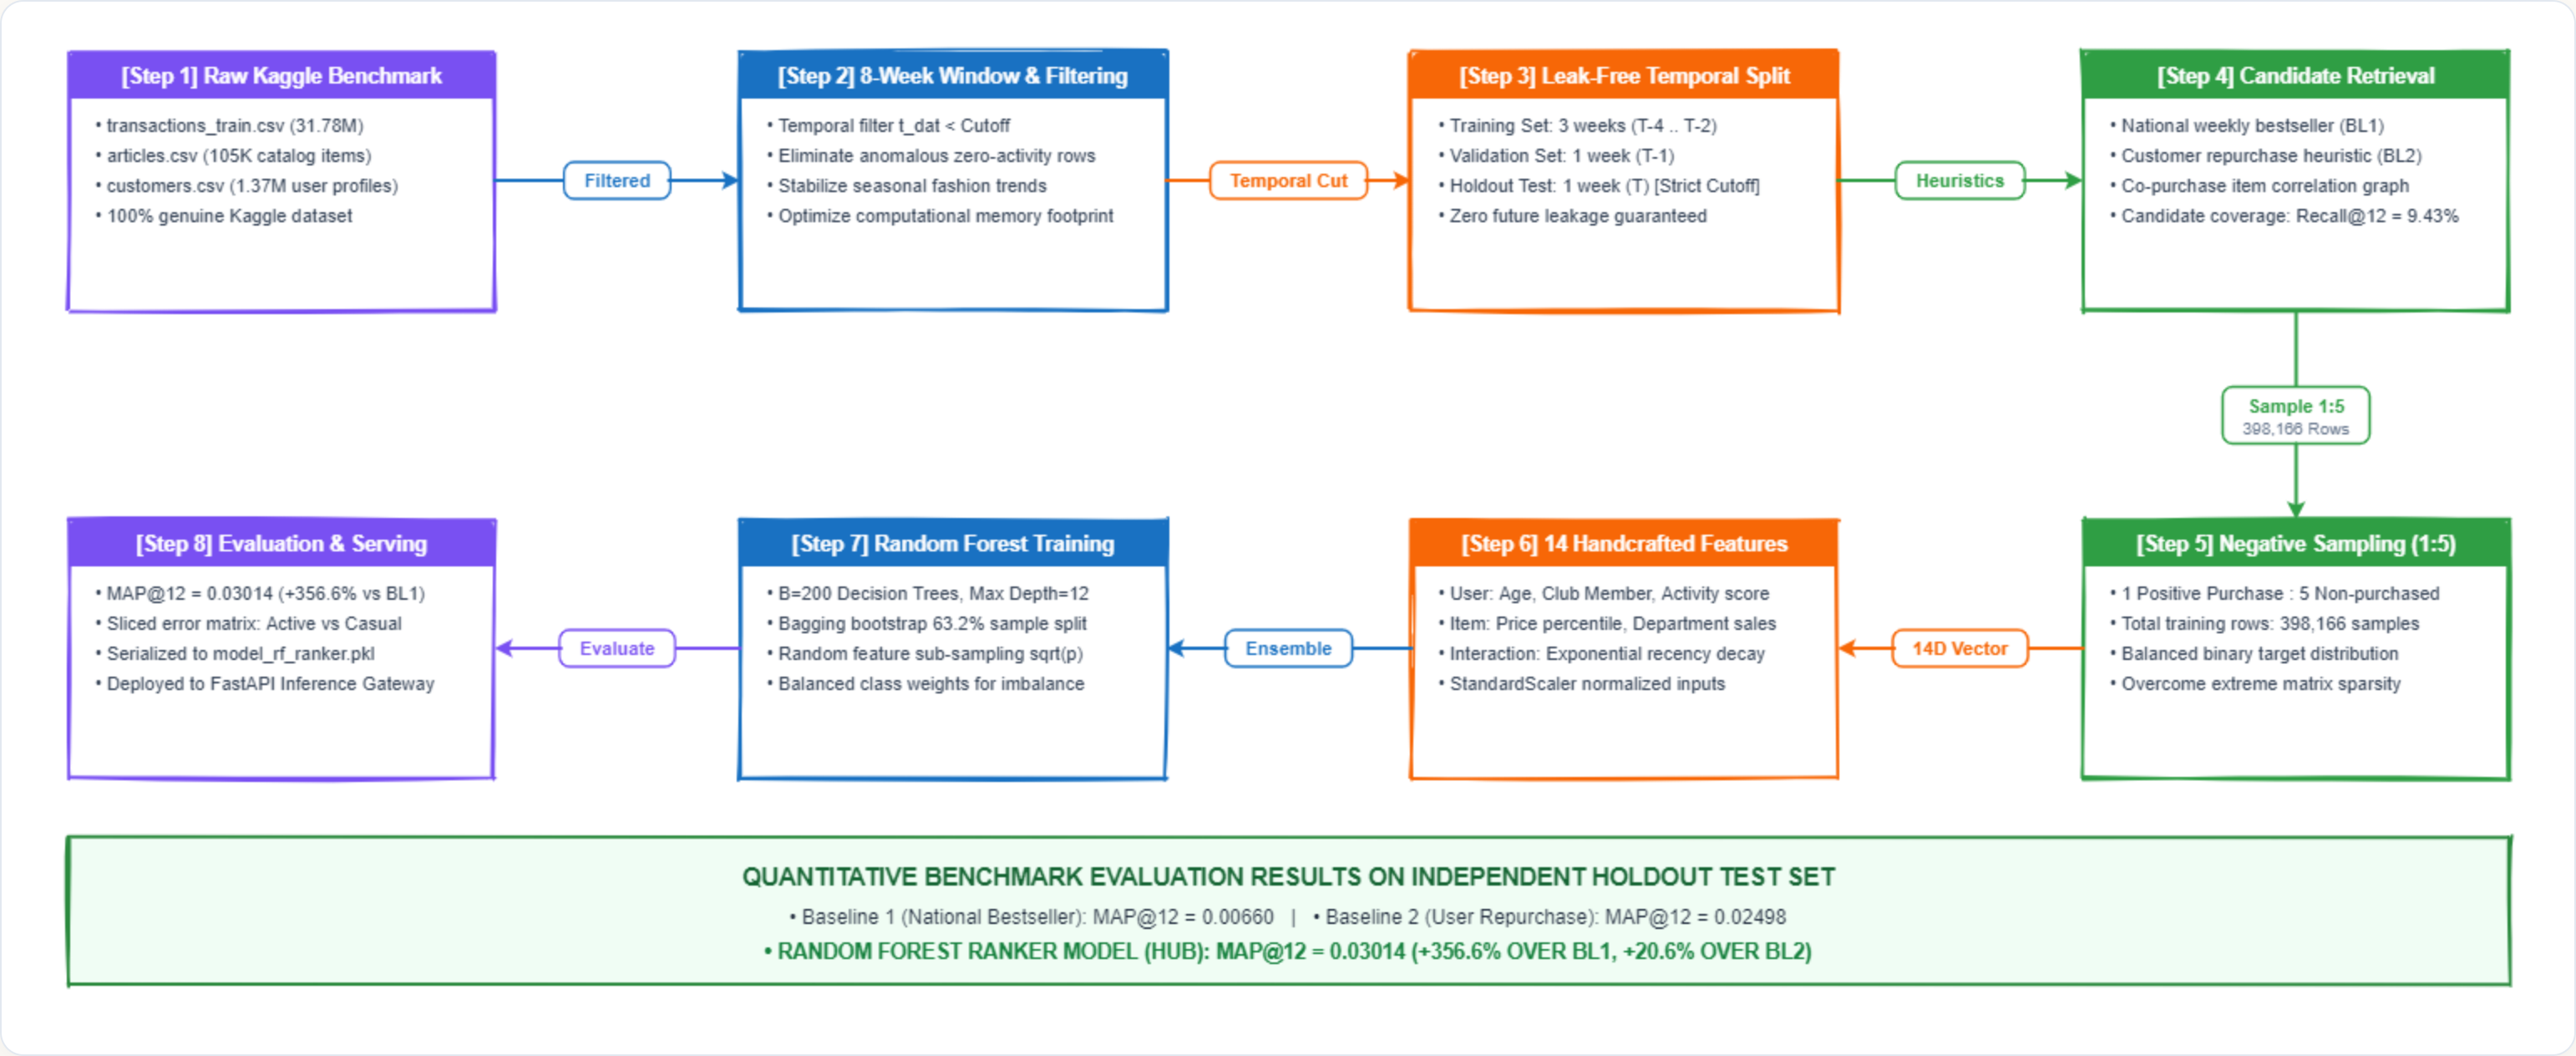
\includegraphics[width=0.95\textwidth]{excalidraw_03_ml_training_pipeline.png}
    \caption{End-to-End MLOps Training Pipeline: Offloaded Kaggle Cloud Execution and Deployment Flow}
    \label{fig:ml_pipeline}
\end{figure}

The retraining pipeline operates asynchronously:
\begin{enumerate}
    \item The FastAPI backend exports fresh customer web purchase events and pushes the executable training payload (\texttt{hub\_pipeline.py}) to Kaggle Cloud Kernels via the Kaggle API.
    \item Execution is monitored through a lightweight status polling thread tracking step-by-step progress ($0\%$ to $100\%$) recorded in \texttt{progress.json}.
    \item Upon job termination, output artifacts (\texttt{summary.json}, \texttt{metrics.json}, \texttt{recs.csv}, \texttt{model\_rf\_ranker.pkl}) are downloaded to the server's versioned directory \texttt{data\_scientist/runs/<run\_id>/}.
\end{enumerate}

\subsection{Six-Step Training Lifecycle Specification}
The execution pipeline is decomposed into six deterministic steps:
\begin{enumerate}
    \item \textbf{Step 1: Temporal Window Partitioning:} Filters transaction logs to the sliding 8-week observation window, eliminating cold records and converting 64-hex identifiers into compact 64-bit integers.
    \item \textbf{Step 2: Candidate Generation:} Executes Algorithm \ref{algo:stage1_retrieval} across repurchase, bestseller, age-cohort, and co-purchase channels to retrieve $C=100$ items per customer.
    \item \textbf{Step 3: Dense Feature Construction:} Generates the 14-dimensional feature vector $\mathbf{x}_{u,i}$ and performs leak-free Standard Scaling ($\mu=0, \sigma=1$).
    \item \textbf{Step 4: Random Forest Model Fitting:} Trains 200 decision trees via multi-threaded CPU parallelization using balanced class weights to offset label sparsity.
    \item \textbf{Step 5: Holdout Benchmark Validation:} Evaluates candidate model predictions on the blind holdout test set against Baseline 1 and Baseline 2.
    \item \textbf{Step 6: Atomic Recommendation Serialization:} Atomically writes the scored Top-12 rankings into the relational \texttt{user\_recommendations} table under an isolated database transaction.
\end{enumerate}

\subsection{Model Degradation Safety Gate Decision Logic}
A catastrophic failure mode in automated retraining systems occurs when a newly trained model suffers metric regression due to anomalous data shifts, degraded features, or extreme noise. To safeguard the production environment, HUB incorporates a formal \textbf{Model Degradation Safety Gate}:

\begin{equation}
    \Delta \operatorname{MAP} = \operatorname{MAP}@12(\mathcal{M}_{\text{candidate}}) - \operatorname{MAP}@12(\mathcal{M}_{\text{production}})
\end{equation}

The deployment decision follows strict mathematical guardrails:
\begin{equation}
    \operatorname{Decision}(\mathcal{M}_{\text{candidate}}) = 
    \begin{cases} 
        \operatorname{AutoDeploy}(\mathcal{M}_{\text{candidate}}) & \text{if } \Delta \operatorname{MAP} \ge 0 \\ 
        \operatorname{RaiseException}(\Delta \operatorname{MAP}) & \text{if } \Delta \operatorname{MAP} < 0 
    \end{cases}
\end{equation}

When $\Delta \operatorname{MAP} < 0$, automatic deployment is instantly halted. The system raises an alert on the Data Scientist \textit{Training Schedule} interface, requiring human-in-the-loop inspection. The engineer may either investigate the anomaly and retain the verified production model (\textit{"Keep Current"}), or provide explicit administrative override (\textit{"Overwrite Anyway"}).

\subsection{Automated Cron Scheduling}
The system registers an automated operating system Cron schedule running daily at \textbf{02:00 AM} (UTC+7). The background daemon aggregates daily sales tallies, triggers the retraining pipeline, checks the degradation gate, and serializes refreshed recommendations before peak morning browsing traffic.
